\documentclass[11pt,a4paper]{article}
\usepackage{graphicx}
\usepackage{amssymb, amsmath}
\usepackage{url}
\usepackage{polski}
\usepackage{subfigure}
\usepackage[utf8]{inputenc} 

\title{Współczesne techniki heurystyczne\\ Sprawozdanie końcowe\\ \large Zastosowanie algorytmu rozmytego do sterowania prędkością samochodu}
\author{Piotr Jastrzębski\\ Marcin Nazimek}
\date{}
\begin{document}
\maketitle

\section{Szczegółowy opis zadania}\label{opis}
Rozważmy poruszający się samochód. W celu stworzenia modelu ruchu bierzemy pod uwagę dwie zmienne wejściowe: PRĘDKOŚĆ i ODLEGŁOŚĆ od jadącego z przodu samochodu oraz jedna zmienna określająca zmianę tego ruchu PRZYSPIESZENIE. Sterowanie odbywać będzie się poprzez zmianę prędkości. Przykładowe możliwe stany to: przyspieszenie, utrzymanie prędkości i hamowanie (ale można przyjąć więcej stanów, np. odległość jest bardzo mała, itp.).

Dla rozpatrywanego przypadku, baza reguł ma postać:
\begin{itemize}
\item IF odległość jest mała AND prędkość jest mała THEN utrzymaj prędkość.
\item IF odległość jest mała AND prędkość jest duża THEN zredukuj prędkość.
\item IF odległość jest duża AND prędkość jest mała THEN zwiększaj prędkość.
\item IF odległość jest duża AND prędkość jest duża THEN utrzymaj prędkość.
\end{itemize}
Zmienne ODLEGŁOŚĆ, PRĘDKOŚĆ i PRZYSPIESZENIE to zmienne lingwistyczne, które mogą przyjmować rozmyte wartości: krótki, długi, mała, duża, utrzymaj, zredukuj i zwiększaj. Projektant ma teraz za zadanie dobrać tak parametry zbiorów rozmytych i obszarów rozważań by odpowiadały one rzeczywistości w jak najlepszym stopniu.

\section{Założenia projektu}\label{zalozenia}
Projekt ma symulować i prezentować wykorzystanie algorytmu logiki rozmytej do sterowania prędkością samochodu w~możliwie największym stopniu odwzorowując rzeczywistość.

W przygotowanym środowisku na potrzeby prezentacji wykorzystane są dwa uproszczone modele reprezentujące samochody -- pierwszy, dalej oznaczany jako $A$, będący samochodem, dla którego przygotowane zostanie sterowanie, oraz samochód $B$, który w sposób niedeterministyczny, ale zgodny z przepisami i realnymi wartościami przyspieszeń, będzie poruszał się przed $A$. Każdy z nich w~danej chwili czasu opisany będzie prędkością bezwzględną. 

Odległość między samochodami wynika wprost z różnic prędkości, a prędkość auta $A$ modyfikowana jest przez wartość wyjścia modułu logiki rozmytej -- przyspieszeniem.

\subsection{Ograniczenia}
Na potrzeby projektu przyjęto następujące ograniczenia:
\begin{itemize}
\item \textbf{Prędkość} - przyjmuje wartości z zakresu $0\div140km/h$ \footnote{Założono, że ruch odbywa się na autostradzie w Polsce.}.
\item \textbf{Przyspieszenie} - jest zmienne w czasie. Kwestią do rozstrzygnięcia pozostaje, czy będzie ono takie samo czy przyjmie różne wartości dla opóźnienia i przyspieszenia. Na bazie zgromadzonych informacji odpowiednie wydaje się przyjęcie wartości przyspieszenia z zakresu $\langle-9\frac{m}{s^2};4\frac{m}{s^2}\rangle$\footnote{Wartości prawdziwe dla suchej nawierzchni.} i~dla aktualnego stanu zaawansowania projektu takie jest wykorzystywane.
\item \textbf{Odległość} - wyrażona w kilometrach dowolną nieujemną liczbą dziesiętną. Testowane jest rozwiązanie, które rozważa niejako dwa stany:
	\begin{itemize}
		\item stan bliski -- do odległości $1 km$, gdzie aktywny jest moduł logiki rozmytej
		\item stan daleki -- powyżej $1km$, gdzie samochód porusza się prędkością autostradową, tak długo, aż nie na trafi w odległości $1 km$ ma poprzedzające auto. Tym samym wartość $1 km$ jest wartością rozgraniczającą niejako nieskończoność od skutecznej odległości działania modułu dystansującego.
	\end{itemize}
\end{itemize}
Każde przekroczenie wartości $0$ świadczy o najechaniu na samochód poprzedzający i~w~końcowej wersji projektu nie ma prawa wystąpić.

\subsection{Stan początkowy}
Przed rozpoczęciem symulacji stan układu (wartości poszczególnych parametrów) mogą być modyfikowane. Ustalane mogą być zarówno prędkość początkowa samochodu $A$ oraz $B$ jak i odległość między nimi. Celem symulacji jest tak sterować parametrami samochodu $A$, aby zachowywał on stałą odległość od poprzedzającego go samochodu nie powodując kolizji (najechania). Aktualnie zaimplementowana funkcjonalność pozwala na dowolne sterowanie prędkością samochodu poprzedzającego.

\section{Implementacja środowiska}
W celu prezentacji działania algorytmu wykorzystywane są funkcjonalności zawarte w programie \emph{Matlab R2011a} wraz z rozszerzeniem \emph{Fuzzy Logic Toolbox}. Moduł ten zapewnia funkcje, narzędzia graficzne i elementy \emph{Simulink} dla systemów bazujących na logice rozmytej. W~zaproponowanym rozwiązaniu bezwzględne prędkości aut prezentowane są na tym samym wykresie pozwalając obserwować proces reakcji samochodu sterowanego modułem logiki rozmytej. Zrzut ekranu przedstawiający środowisko symulacji przedstawiono na rysunku \ref{img:simulink}.

\begin{figure}
\centering 
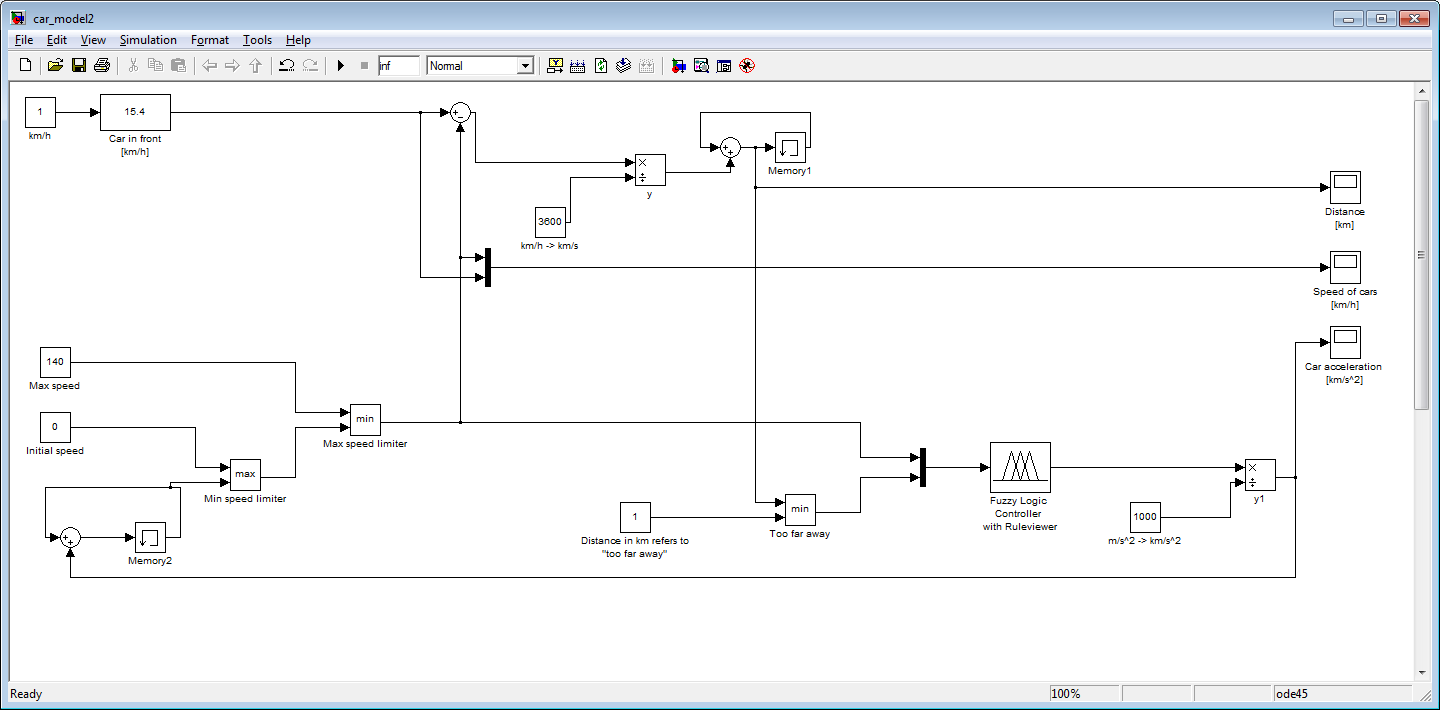
\includegraphics[width=0.8\textwidth]{simulink.png}
\caption{Środowisko symulacji ruchu samochodów} 
\label{img:simulink}
\end{figure}

\section{Implementacja logiki rozmytej}
Obok schematu \emph{Simulink} symulującego środowisko najważniejszą częścią układu jest moduł odpowiedzialny za implementację logiki rozmytej. Moduł ten (Fuzzy Logic Controller) został zdefiniowany w~następujący sposób:

\subsection{Fuzzyfikacja (rozmycie)}
Rozmywanie polega na określeniu stopnia przynależności danej wartości wielkości wejściowej do każdego z~odpowiadających jej zbiorów rozmytych pokrywających zakres możliwych wartości wejściowych. Operacja ta sprowadza się do obliczaniu wartości funkcji. Wartości wejściowe opisywane są funkcją trójkątną o wzorze:

\begin{equation}
f(x)=\left\{ 
  \begin{array}{l l}
    0, & \quad x\leq a\\
    \frac{x-a}{b-a}, &\quad a\leq x \leq b \\
    \frac{c-x}{c-b}, &\quad b\leq x \leq c \\
    0, &\quad c\leq x\\
  \end{array} \right.
  \label{trojkat}
  \end{equation}

\begin{itemize}
\item Prędkość (\emph{speed}) - określona jest funkcją trójkątną o parametrach:
\begin{itemize}
\item prędkość niska (\emph{low}) $(a=-140, b=0, c=140)$
\item prędkość wysoka (\emph{high}) $(a=0, b=140, c=280)$
\end{itemize}

\item Odległość (\emph{distance}) - określona również funkcją trójkątną, gdzie:
\begin{itemize}
\item odległość mała (\emph{short}) $(a=-1, b=0, c=1)$
\item odległość duża (\emph{long}) $(a=0.5, b=1, c=2)$
\end{itemize}

\end{itemize}

\subsection{Zastosowanie operatorów logiki rozmytej do określenia stopnia, w jakim spełniona jest  
przesłanka w każdej z reguł}
Jak widać w~punkcie \ref{opis} w~bazie reguł znajduje się jedynie funkcja logicznej koniunkcji (\emph{AND}) warunków. Funkcja dla koniunkcji ustalona została jako wartość minimalna (\emph{min}) elementów składowych poprzednika implikacji.

\subsection{Zastosowanie metody implikacji}
Funkcja implikacja to również funkcja minimalnej wartości - \emph{min}.

\subsection{Agregacja wszystkich wyjść}
Funkcja agregująca wszystkie wyjścia bierze pod uwagę wartość maksymalną (\emph{max}) spośród wszystkich następników reguł. Funkcje wyjść zdefiniowane są jako:
\begin{itemize}
\item Przyspieszenie (\emph{acceleration}) - określone funkcjami o różnym przebiegu:
\begin{itemize}
\item zmniejsz (\emph{decrease}) $(a=0.15, b=0.6, c=-9)$ (f. dzwonowa, jak we wzorze \ref{dzwon})
\item utrzymuj (\emph{maintain}) $(a=-0.4, b=0, c=0.4)$ (f. trójkątna, jak we wzorze  \ref{trojkat})
\item zwiększ (\emph{increase}) $(a=0, b=1.5, c=4, d=10)$ (f. trapezoidalna, jak we wzorze \ref{trapez})
\end{itemize}
\end{itemize}

\subsection{Schemat wnioskowania rozmytego}
Wykorzystany został schemat wnioskowania rozmytego \emph{Mamdani}, który to charakteryzuje się łączeniem następników każdej reguły poprzez
operator agregacji a następnie przeprowadzaniem defuzzyfikacji w~celu otrzymania odpowiedzi systemu. Toolbox logiki rozmytej pozwalał także na wybranie modelu typu \emph{Sugeno}, w~którym następnik każdej reguły jest liniową kombinacją wejść systemu. Wyjście systemu jest ważoną kombinacją liniową następników reguł definiujących system.

\subsection{Defuzzyfikacja (wyostrzanie)}
Wartość wyostrzana jest wyznaczana funkcją \emph{centroid} - jest to punkt na osi argumentów będący przecięciem linii równowagi powierzchni pod krzywą z osią argumentów. Wzór funkcji składowych: trójkątnej przedstawiono jako \ref{trojkat}, dzwonowej jako \ref{dzwon}, a~funkcji trapezoidalnej jako \ref{trapez}.

\begin{equation}f(x)=\frac{1}{ 1+{|\frac{x-c}{a}|}^{2b} }
\label{dzwon}\end{equation}

\begin{equation}
f(x)=\left\{ 
  \begin{array}{l l}
    0, & \quad x\leq a\\
    \frac{x-a}{b-a}, &\quad a\leq x \leq b \\
    1, &\quad b\leq x \leq c \\
    \frac{d-x}{d-c}, &\quad c\leq x \leq d \\
    0, &\quad c\leq x\\
  \end{array} \right.
  \label{trapez}
\end{equation}

\begin{figure}
\label{img:fuzzy}
\centering
\mbox{
\subfigure[Funkcja wejściowa prędkości]{\label{img:x1}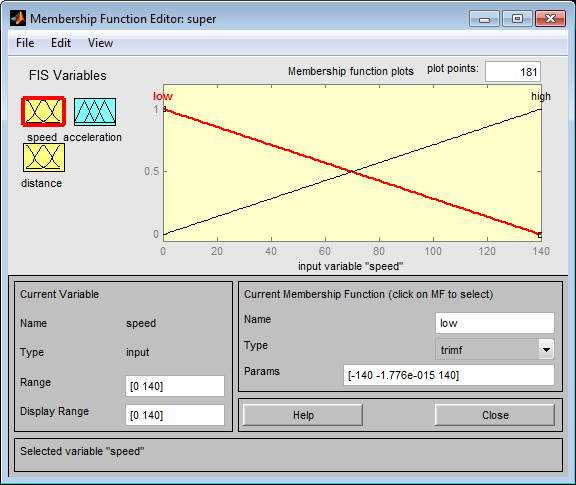
\includegraphics[width=0.40\textwidth]{input.png}} \quad
\subfigure[Funkcje wejściowa odległości]{\label{img:x2}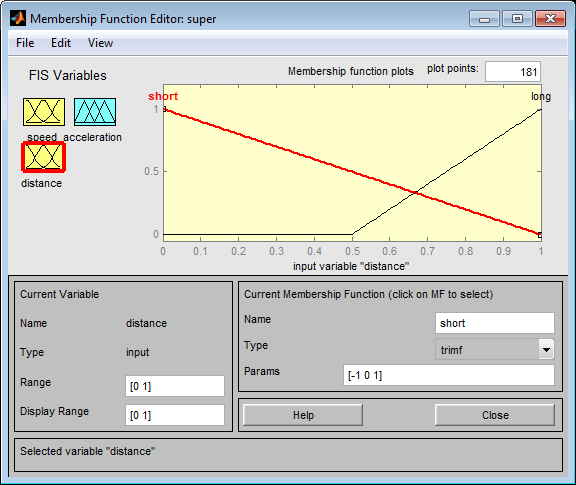
\includegraphics[width=0.40\textwidth]{input2.png}}
}
\mbox{
\subfigure[Funkcja wyjściowa]{\label{img:x3}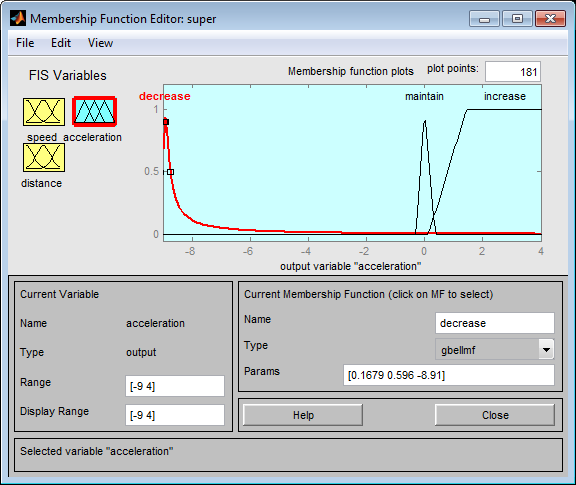
\includegraphics[width=0.40\textwidth]{output.png}}\quad
\subfigure[Płaszczyzna funkcji wyjściowej]{\label{img:x4}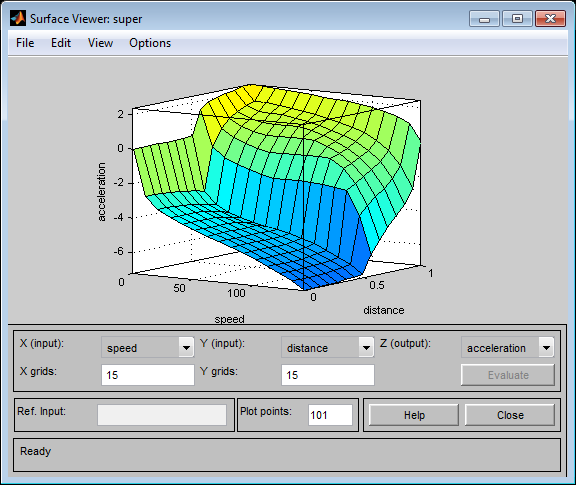
\includegraphics[width=0.40\textwidth]{surface.png}} 
}
\caption{Porównanie przykładowych kształtów funkcji oraz płaszczyzny wartości przyspieszenia w zależności od prędkości i~odległości.}
\end{figure} 

\section{Wyniki, testy poprawności i jakości algorytmów}
Proces testowania polegał na wielokrotnym uruchamianiu symulacji w~module \emph{Simulink}. Każda symulacja trwała przynajmniej minutę i~realizowała oddzielny scenariusz odzwierciedlający rzeczywistą sytuację na drodze (korek, pościg za samochodem albo normalny ruch uliczny). Wynikiem koniecznym zaliczenia testów było nieosiągnięcie ujemnej wartości odległości między samochodami, co sugerowałoby wystąpienie kolizji. Wyniki potwierdzające skuteczność sterowania można zobaczyć na rysunkach \ref{img:test1}, \ref{img:test2} oraz \ref{img:test3}.

\begin{figure}
\centering
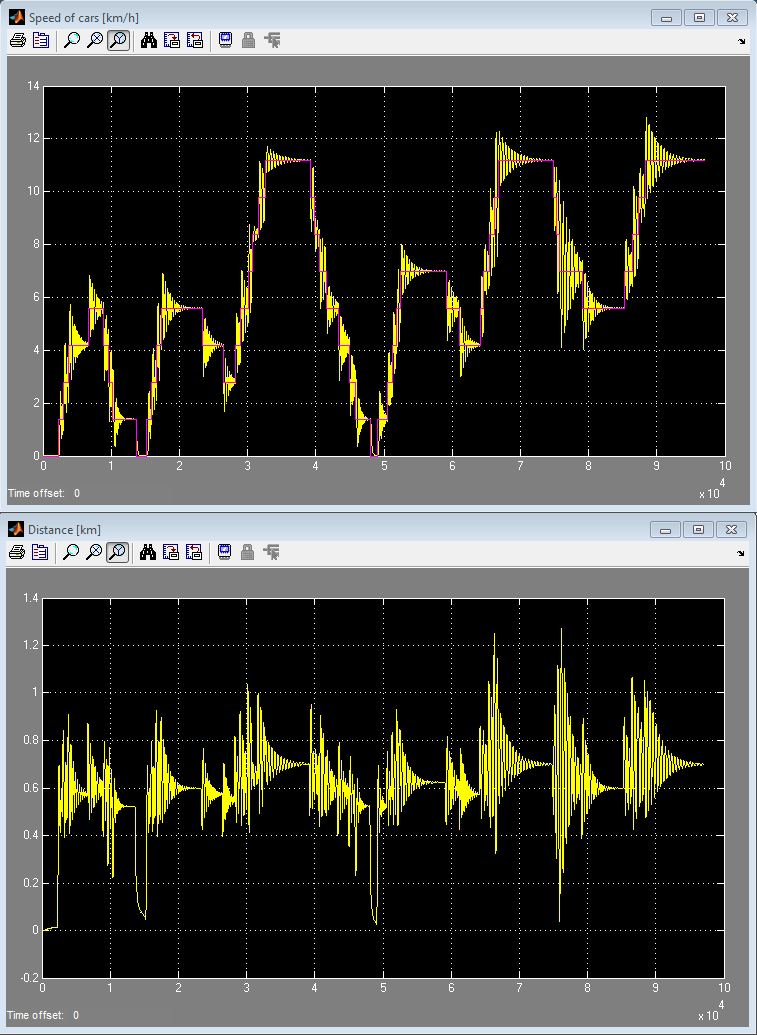
\includegraphics[width=0.95\textwidth]{traffic.png}
\caption{Test 1 - korek uliczny} 
\label{img:test1}
\end{figure}

\begin{figure}
\centering
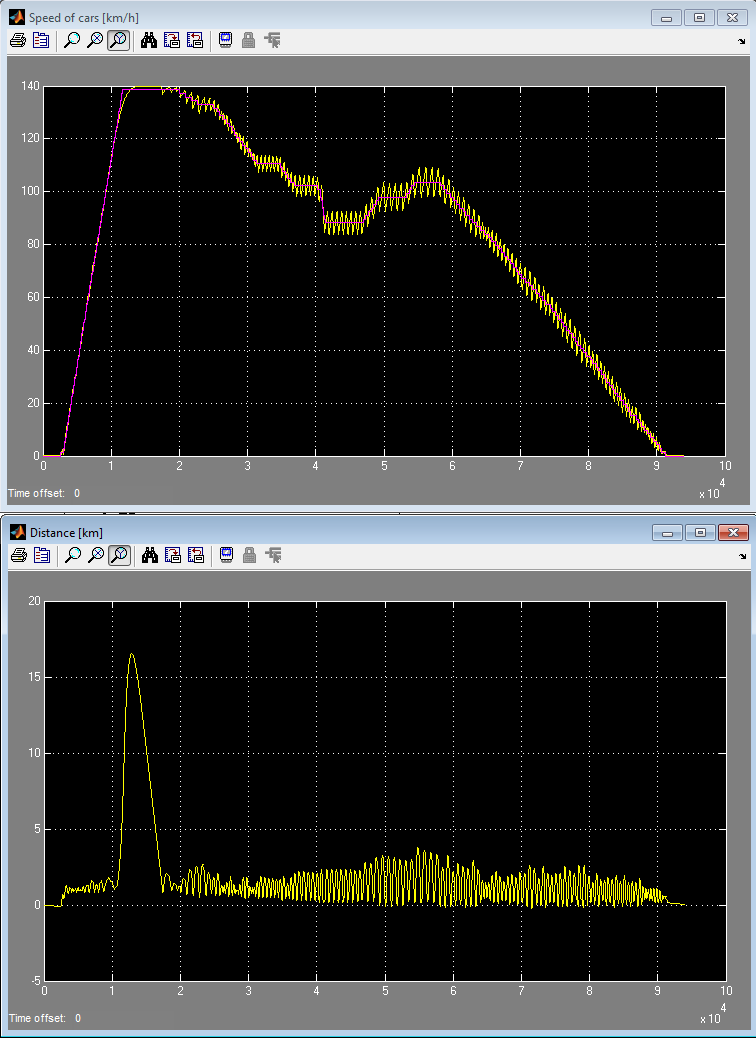
\includegraphics[width=0.95\textwidth]{highSpeedChase.png}
\caption{Test 2 - pościg za szybkim samochodem} 
\label{img:test2}
\end{figure}

\begin{figure}
\centering
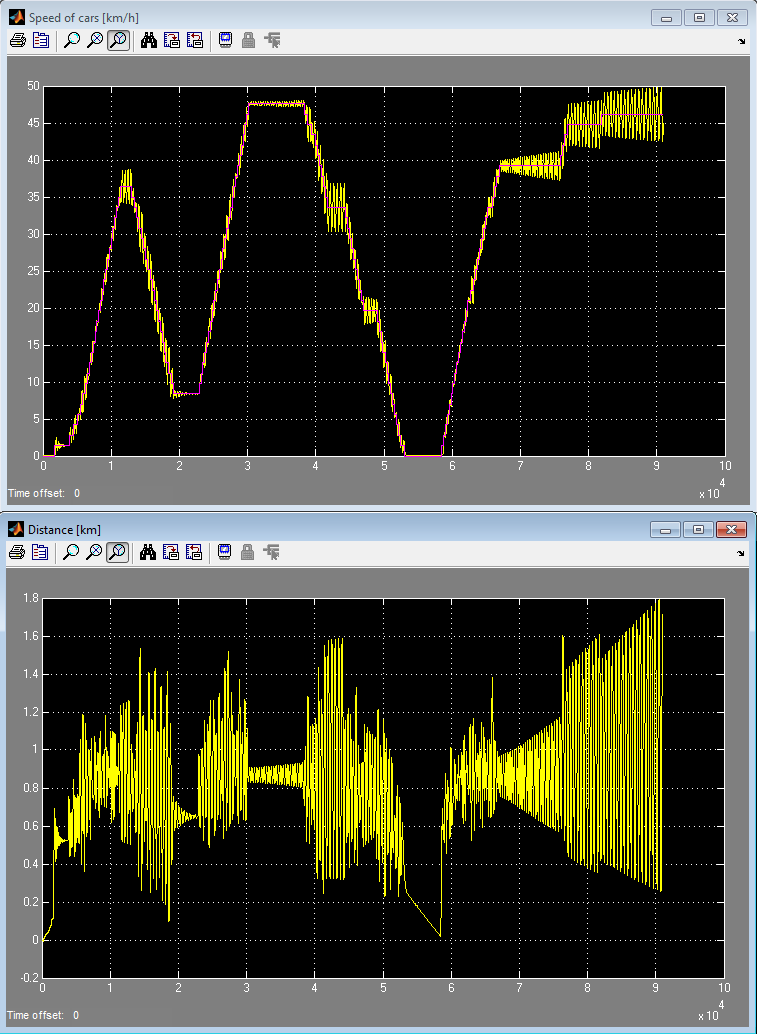
\includegraphics[width=0.95\textwidth]{city.png}
\caption{Test 3 - normalny ruch miejski} 
\label{img:test3}
\end{figure}

\section{Wnioski}
Wyniki, a szczególnie wykresy zgromadzone podczas pracy algorytmu, przywołują na myśl sterowanie z wykorzystaniem regulatorów PID. Analiza wykresów pozwala założyć, że moduł sterowania prędkością samochodu działa prawidłowo i~spełnia zasady bezpieczeństwa nie dopuszczając do wystąpienia sytuacji najechania.

\begin{thebibliography}{9}
	\bibitem{manual}
	\emph{Fuzzy Logic Toolbox User’s Guide}\\
	\url{http://www.mathworks.com/help/pdf_doc/fuzzy/fuzzy.pdf}

	\bibitem{engApp}
	Ross T., \emph{Fuzzy Logic with Engineering Applications}

	\bibitem{opis}
	Rykaczewski K., \emph{Systemy rozmyte i ich zastosowania}\\
	\url{http://math.uni.lodz.pl/~fulmanp/zajecia/ssn/materialy/duszek.pdf}

	\bibitem{ieee1}
	Mamat M., Ghani N. M.,\emph{Fuzzy Logic Controller on Automated Car Braking System}, IEEE International Conference on Control and Automation, 2009. ICCA 2009. 

	\bibitem{ieee2}
	Khodayari, A., Kazemi, R., Ghaffari, A., Braunstingl, R., \emph{Design of an improved fuzzy logic based model for prediction of car following behavior}, IEEE International Conference on Mechatronics (ICM), 2011 

	\bibitem{ieee3}
	Sato, T., Akamatsu, M., Pengjun Zheng, McDonald, M., \emph{Comparison of car following behavior between UK and Japan}, ICCAS-SICE, 2009
	
	\bibitem{simulink}
	\emph{Simulating Dynamic Systems}\\
	\url{http://www.mathworks.com/help/simulink/ug/simulating-dynamic-systems.html}
\end{thebibliography}
\end{document}
